%%%%%%%%%%%%%%%%%%%%%%%%%%%%%%%%%%%%%%%%%
% Journal Article
% LaTeX Template
% Version 1.4 (15/5/16)
%
% This template has been downloaded from:
% http://www.LaTeXTemplates.com
%
% Original author:
% Frits Wenneker (http://www.howtotex.com) with extensive modifications by
% Vel (vel@LaTeXTemplates.com)
%
% License:
% CC BY-NC-SA 3.0 (http://creativecommons.org/licenses/by-nc-sa/3.0/)
%
%%%%%%%%%%%%%%%%%%%%%%%%%%%%%%%%%%%%%%%%%

%----------------------------------------------------------------------------------------
%	PACKAGES AND OTHER DOCUMENT CONFIGURATIONS
%----------------------------------------------------------------------------------------

%\documentclass[10pt]{article} % Single column

\documentclass[colorinlistoftodos,twoside,twocolumn,10pt]{article} % Two column

\usepackage{blindtext} % Package to generate dummy text throughout this template 

\usepackage[sc]{mathpazo} % Use the Palatino font
\usepackage[T1]{fontenc} % Use 8-bit encoding that has 256 glyphs
\linespread{1.05} % Line spacing - Palatino needs more space between lines
\usepackage{microtype} % Slightly tweak font spacing for aesthetics

\usepackage[spanish]{babel} % Language hyphenation and typographical rules

\usepackage[hmarginratio=1:1,top=20mm,columnsep=15mm, left=12mm, right=12mm, bottom=25mm]{geometry} % Document margins
\usepackage[hang, small,labelfont=bf,up,textfont=it,up]{caption} % Custom captions under/above floats in tables or figures
\usepackage{booktabs} % Horizontal rules in tables

\usepackage{lettrine} % The lettrine is the first enlarged letter at the beginning of the text

\usepackage{enumitem} % Customized lists
\setlist[itemize]{noitemsep} % Make itemize lists more compact

\usepackage{abstract} % Allows abstract customization
\renewcommand{\abstractnamefont}{\normalfont\bfseries} % Set the "Abstract" text to bold
\renewcommand{\abstracttextfont}{\normalfont\small\itshape} % Set the abstract itself to small italic text

\usepackage{titlesec} % Allows customization of titles
\renewcommand\thesection{\Roman{section}} % Roman numerals for the sections
\renewcommand\thesubsection{\roman{subsection}} % roman numerals for subsections
\titleformat{\section}[block]{\large\scshape\centering}{\thesection.}{1em}{} % Change the look of the section titles
\titleformat{\subsection}[block]{\large}{\thesubsection.}{1em}{} % Change the look of the section titles

\usepackage{fancyhdr} % Headers and footers
\pagestyle{fancy} % All pages have headers and footers
\fancyhead{} % Blank out the default header
\fancyfoot{} % Blank out the default footer
\fancyhead[C]{Music Genre Classifier} % Custom header text
\fancyfoot[RO,LE]{\thepage} % Custom footer text

\usepackage{titling} % Customizing the title section

\usepackage[colorlinks]{hyperref} % For hyperlinks in the PDF

\usepackage{graphicx} % For images
\usepackage{subcaption}

\usepackage{pifont} % bullets

\usepackage{amsmath}


% Keywords command
\providecommand{\keywords}[1]
{
	\small	
	\vspace{0.5em}
	\noindent \textbf{\textit{Palabras clave --- }} #1
}

%----------------------------------------------------------------------------------------
%	TITLE SECTION
%----------------------------------------------------------------------------------------

\setlength{\droptitle}{-4\baselineskip} % Move the title up

\pretitle{\begin{center}\Huge\bfseries} % Article title formatting
	\posttitle{\end{center}} % Article title closing formatting
\title{\normalsize{Proyecto Final de Aprendizaje de M\'aquina}\\
	\Huge\bfseries Music Genre Classifier\\
} % Article title
\author{% 
	\normalsize\textsc{Integrantes:}\\
	\normalsize\textsc{Marcos Tirador Del Riego  C-411}\\
	\normalsize\textsc{Leandro Rodr\'iquez Llosa  C-411}\\
	\normalsize\textsc{Victor Manuel Amador Sosa C-412}\\
	\normalsize\textsc{Francisco Ayra Caceres C-412}\\
	\normalsize\textsc{Ra\'ul Beltr\'an G\'omez C-412}\\
	\normalsize\textsc{Niley Gonz\'alez Ferrales  C-411}\\
	\normalsize\textsc{Arian Pazo Valido  C-311} \\[2ex]
	\small Cuarto a\~no. Ciencias de la Computaci\'on. \\ % institution
	\small Facultad de Matem\'atica y Computaci\'on, Universidad de La Habana, Cuba \\ % institution
}
\date{\footnotesize Junio 2023 } % Leave empty to omit a date


% Abstract configurations
\renewenvironment{abstract}
{\small
	\begin{center}
		\bfseries \abstractname\vspace{-.5em}\vspace{0pt}
	\end{center}
	\list{}{
		\setlength{\leftmargin}{0.9cm}%
		\setlength{\rightmargin}{\leftmargin}%
	}%
	\item\relax}
{\endlist}


\usepackage{todonotes} % \TODO
\usepackage{listings} % Code listings
\usepackage{xcolor}
\definecolor{backcolour}{rgb}{0.95,0.95,0.92}

\newcommand{\csl}[1]{\colorbox{backcolour}{\texttt{#1}}}

\newcommand{\imgcaption}[2]{\tiny \textbf{Figura #1.} #2.}

\newcommand{\mgc}[2][]{\colorbox{backcolour}{\texttt{\_\_#2\_\_#1}}}

\newcommand{\mgccapt}[1]{\texttt{\_\_#1\_\_}}

% Hyperlinks configurations
\hypersetup{
	colorlinks=true,
	linkcolor=black,
	filecolor=magenta,      
	urlcolor=cyan,
	pdftitle={Overleaf Example},
	pdfpagemode=FullScreen,
}

%----------------------------------------------------------------------------------------

\begin{document}
	% Print the title
	\maketitle

    \selectlanguage{spanish}
	\pagenumbering{gobble}
	\begin{abstract}

La clasificaci\'on de g\'eneros musicales juega un papel crucial en las aplicaciones modernas de procesamiento de se\~nales de audio digital. En este estudio, proponemos varios enfoques de aprendizaje autom\'atico para categorizar con precisi\'on pistas de m\'usica en g\'eneros predefinidos. Cada enfoque utiliza diversos conjuntos de caracter\'isticas que se pueden extraer de las canciones; desde los comunes: MFCC, se\~nal de audio directa; hasta caracter\'isticas poco exploradas en este problema: letra de la canci\'on, Transformada de Wavelet. Para evaluar los modelos utilizamos el dataset de referencia en el campo, GTZAN. En los resultados obtenidos destaca que la letra de la canci\'on no aporta mucho a la clasificaci\'on, al menos en el dataset utilizado. Los otros modelos muestran resultados consistentes con el estado del arte, con una precisi\'on entre $75\%$ y $80\%$

		\vspace{1em}
		\keywords{ 
			aprendizaje autom\'atico \textbf{$\cdot$} clasificaci\'on \textbf{$\cdot$}  g\'eneros musicales \textbf{$\cdot$} MFCC  \textbf{$\cdot$} CNN  \textbf{$\cdot$} Conv1D \textbf{$\cdot$} transformada wavelet discreta \textbf{$\cdot$} transformada wavelet compleja de doble \'arbol  \textbf{$\cdot$} encoder  \textbf{$\cdot$} letra de canciones 
		}

	\end{abstract}
	
	%----------------------------------------------------------------------------------------
	%	ARTICLE CONTENTS
	%----------------------------------------------------------------------------------------
	
	\section{Introducci\'on}
	La clasificaci\'on autom\'atica de g\'eneros musicales se ha vuelto cada vez m\'as importante debido a la gran cantidad de m\'usica digitalizada disponible en la actualidad. El etiquetado de g\'eneros preciso permite una organizaci\'on, recuperaci\'on y recomendaci\'on eficientes de canciones, allanando el camino para experiencias personalizadas en servicios multimedia. La identificaci\'on de g\'eneros es \'util para crear listas de reproducci\'on personalizadas, analizar las preferencias de los oyentes, recomendar artistas/canciones similares, detectar material con derechos de autor e identificar estados de \'animo asociados con ciertos g\'eneros. Sin embargo, a pesar de la gran cantidad de soluciones y avances propuestos en el procesamiento de se\~nales musicales, persisten varios problemas para lograr sistemas de reconocimiento de g\'enero robustos y eficientes.

En primer lugar, la definici\'on de g\'eneros musicales sigue siendo controvertida, ya que la percepci\'on humana var\'ia mucho. Estas interpretaciones subjetivas conducen a anotaciones inconsistentes  y l\'imites ambiguos entre g\'eneros. Esta falta de consenso impide el desarrollo de modelos confiables capaces de generalizar a trav\'es de diferentes conjuntos de datos.

Aunque los g\'eneros se derivan de influencias culturales, hist\'oricas, sociales, geogr\'aficas, tecnol\'ogicas y creativas, por lo general se reducen a etiquetas binarias. Sin embargo, muchos estilos comparten atributos y se superponen, lo que los hace dif\'iciles de distinguir. Adem\'as, los artistas mezclan con frecuencia diferentes g\'eneros, lo que agrega complejidad al proceso de clasificaci\'on.

En segundo lugar, la disponibilidad limitada de datos etiquetados de alta calidad plantea un gran desaf\'io cuando se entrenan algoritmos de aprendizaje autom\'atico para la clasificaci\'on de g\'eneros musicales. Debido al extenso tiempo que se requiere para etiquetar manualmente las pistas con g\'eneros espec\'ificos, muchos investigadores recurren a conjuntos de datos peque\~nos o sint\'eticos, lo que lleva a modelos sobreajustados o inadecuados. Adem\'as, la obtenci\'on de colecciones m\'as importantes a menudo implica derechos de licencia o barreras t\'ecnicas, lo que dificulta la accesibilidad y la reproducibilidad.

Por \'ultimo, los enfoques actuales de aprendizaje profundo se basan en gran medida en procedimientos de preentrenamiento computacionalmente costosos, lo que los hace intensivos en recursos. Los trabajos existentes suelen utilizar servicios en la nube o potentes GPU, lo que dificulta la implementaci\'on pr\'actica sin hardware especializado o recursos financieros. 
	  

\section {An\'alisis del problema}
\subsection {CNN-MFCC model}
El problema que se pretende resolver es la clasificaci\'on de g\'eneros musicales utilizando redes neuronales convolucionales como modelo de aprendizaje y el feature MFCC como caracter\'istica extraida de los audios.
Los MFCC se utilizan com\'unmente en el procesamiento de se\~nales de audio y voz para extraer caracter\'isticas que se pueden utilizar en diversas aplicaciones, como el reconocimiento de voz y la clasificaci\'on de g\'eneros musicales. Se basan en la observaci\'on de que el sistema auditivo humano es m\'as sensible a los cambios de frecuencia en las frecuencias m\'as bajas en comparaci\'on con las frecuencias m\'as altas. La escala de frecuencia Mel es una transformaci\'on no lineal de la frecuencia que aproxima la respuesta del sistema auditivo humano al sonido. La raz\'on por la que se utilizan los MFCC es que son una representaci\'on compacta del envolvente espectral de la se\~nal de audio, lo cual es particularmente \'util cuando se trata con grandes cantidades de datos de audio.
Uno de los enfoques m\'as populares y efectivos para abordar la clasificaci\'on de g\'eneros musicales es utilizar los coeficientes cepstrales de frecuencia mel (MFCC) como caracter\'isticas para representar las se\~nales de audio.

Los MFCC son una t\'ecnica poderosa de extracci\'on de caracter\'isticas para el procesamiento de se\~nales de audio y voz y se han utilizado ampliamente en una variedad de aplicaciones, incluyendo el reconocimiento de voz, la clasificaci\'on de g\'eneros musicales y m\'as.
Uno de los enfoques m\'as populares y efectivos para abordar el problema de clasificaci\'on de g\'eneros musicales es utilizar estos coeficientes cepstrales de frecuencia mel (MFCC) como caracter\'isticas para representar las se\~nales de audio.

\subsection {Autoencoder}
Una de las ideas implementadas para hacer uno de los clasificadores de nuestro ensemble combina an\'alisis de la letra con un embedding y de la m\'usica con un encoder. La idea de este modelo es concatenar los vectores resultantes de estos procesamientos y clasificar en base a esta combinaci\'on de features.

\section {An\'alisis del estado del arte}
\subsection {CNN-MFCC model}
\textit{Machine Learning and Deep Learning methods for music genre Classification} \cite{Machine Learning and Deep Learning methods for music genre Classification} de Ruslan Gokhman es un art\'iculo de investigaci\'on que compara el rendimiento de diferentes arquitecturas de redes neuronales profundas para la clasificaci\'on de g\'eneros musicales. [3]
En su estudio, Ruslan compara el rendimiento de varias arquitecturas de redes neuronales profundas en una tarea de clasificaci\'on de g\'eneros musicales. Utiliza como conjunto de datos la dataset GTZAN. Ruslan eval\'ua el rendimiento de 2 tipos arquitecturas de redes neuronales profundas: redes neuronales convolucionales (CNN) y redes neuronales recurrentes (RNN).

Se aprecia que la arquitectura CNN supera a la mayor parte del resto de las arquitecturas obteniendo un accuracy de 0.84.
Resultados como este sugiere que las CNN pueden ser particularmente adecuadas para esta tarea de clasificaci\'on de audios.

\subsection {Autoencoder}
Como realmente no se pretend\'ia lograr obtener resultados directamente a partir del encoder, se investig\'o en la direcci\'on de autoencoders de im\'agenes y autoencoders en general. Principalmente utilizando ideas de \textit{An Introduction to Autoencoders} \cite{michelucci2022introduction} y \textit{Autoencoders} \cite{bank2021autoencoders}.

\section {Features}
\subsection {CNN-MFCC model}
Para el entrenamiento de este modelo se utiliza el feature MFCC. Este feature es una caracter\'istica extra\'ida de los audios popularmente utilizado para el an\'alisis de los mismos.

La raz\'on por la que se utilizan los MFCC para entrenar el modelo es que son una representaci\'on compacta del espectro de la se\~nal de audio, lo que es particularmente \'util cuando se trabaja con grandes cantidades de datos de audio. Para calcular los MFCC, primero se segmenta la se\~nal de audio en marcos cortos y se aplican una serie de operaciones matem\'aticas a cada marco, incluyendo pre\'enfasis, enventanamiento, transformada de Fourier y compresi\'on logar\'itmica, que juntas crean un conjunto de caracter\'isticas que capturan las caracter\'isticas m\'as importantes de la se\~nal de audio.

Los MFCC se pueden representar como una matriz donde cada fila corresponde a un marco particular de la se\~nal de audio, y cada columna representa un MFCC particular.

Para la extracci\'on de MFCC en la pr\'actica se utiliza la biblioteca de python librosa, la misma posee m\'odulos espec\'ificos para la extracci\'on de la caracter\'istica MFCC de un audio.

\begin{figure}[h!] % Start the main figure environment
	\centering
	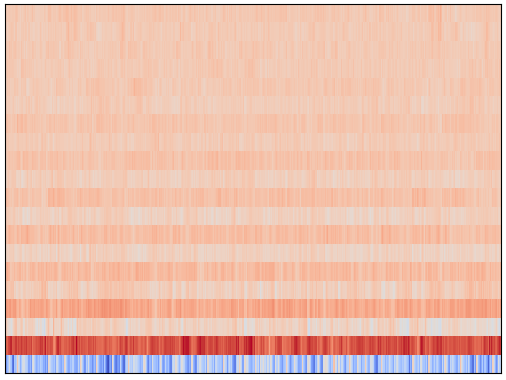
\includegraphics[width=8cm]{mfcc.png}
	\caption{MFCC sample image}
\end{figure}

\subsection {Embedding MFCC (autoencoder)}
Para el entrenamiento del modelo de VisionLang se usa el feature Embedding MFCC, que se halla a partir de pasar la feature MFCC anteriormente mencionada por el encoder generado a partir del autoencoder. Esta feature asocia a cada canci\'on a partir de su MFCC una representaci\'on compacta, solo $500$ dimensiones, de su m\'usica intentando guardar la mayor cantidad de informaci\'on posible de la misma.

\section{modelos}
\subsection {CNN-MFCC model}
Nuestro modelo se basa en redes neuronales convolucionales para tratar con las im\'agenes de MFCC. Estas redes est\'an dise\~nadas espec\'ificamente para detectar patrones y caracter\'isticas en im\'agenes, lo que las hace muy \'utiles en problemas de clasificaci\'on y reconocimiento de objetos. Las redes neuronales convolucionales son muy \'utiles para el procesamiento de im\'agenes porque son capaces de aprender patrones y caracter\'isticas de manera autom\'atica. Esto significa que no se necesita un conocimiento experto para dise\~nar los filtros o caracter\'isticas que se utilizan para procesar las im\'agenes, ya que la red es capaz de aprenderlos a partir de los datos de entrenamiento.

La arquitectura de una CNN se compone de varias capas de procesamiento, incluyendo capas de convoluci\'on y de pooling que permiten extraer caracter\'isticas relevantes de las im\'agenes de entrada. La capa de convoluci\'on es la que aplica un filtro o kernel a la imagen de entrada para detectar patrones espec\'ificos, como bordes, l\'ineas o texturas. La capa de pooling reduce la resoluci\'on de la imagen de salida, lo que ayuda a reducir el n\'umero de par\'ametros que deben entrenarse y a evitar el sobreajuste. Tambi\'en se usan capas independientemente de la necesidad del modelo, como capas para aplanar las im\'agenes a un vector, capas densas para pasarle lo que se detecto en las anteriores y ajustar pesos, y capas de activaci\'on.\\


\textbf{\large Arquitectura de capas del modelo}
\begin{itemize}
	\item Capa de entrada input: recibe la la imagen con tama\~no 256x192 y 3 filtros RGB.(256,192,3).

\item Capa Conv2D: recibe la capa input anterior y devuelve datos de tama\~no (256,192,64), aplica 64 filtros a la imagen.

\item Capa AveragePooling2D: recibe datos de tama\~no (256,192,64) y devuelve la imagen reducida en (2,2), devuelve datos de tama\~no (128,96,64).

\item Capa Conv2D: recibe datos de tama\~no (128,96,64) y devuelve datos de tama\~no (128,96,128), aplica 128 filtros a la imagen.

\item Capa AveragePooling2D recibe datos de tama\~no (128,96,128) y devuelve la imagen reducida en (2,2), devuelve datos de tama\~no (64,48,128).

\item Capa Conv2D: recibe datos de tama\~no (64,48,128) y devuelve datos de tama\~no (64,48,256), aplicando 256 filtros a la imagen.

\item Capa GlobalAveragePooling2D: recibe datos de tama\~no (128,96,128) y devuelve un vector 1D \cite{Machine Learning and Deep Learning methods for music genre Classification} de tama\~no 256, con una salida por cada filtro.

\item Capa Dense de 256 neuronas: recibe los datos de la salida de la capa anterior y los procesa con la funci\'on de activaci\'on RELU.

\item Capa Dense de 128 neuronas: recibe los datos de la salida de la capa anterior y los procesa con la funci\'on de activaci\'on RELU.

\item Capa Dense de 64 neuronas: recibe los datos de la salida de la capa anterior y los procesa con la funci\'on de activaci\'on RELU.

\item Capa Dense de 32 neuronas: recibe los datos de la salida de la capa anterior y los procesa con la funci\'on de activaci\'on RELU.

\item Capa Dense de 10 neuronas: recibe los datos de la salida de la capa anterior y los procesa con la funci\'on de activaci\'on softmax para determinar la salida de tipo clasificaci\'on.
\end{itemize}


\begin{figure}[h!] % Start the main figure environment
	\centering
	\includegraphics[width=8cm]{CNN.png}
	\caption{CNN Model}
\end{figure}
\subsection {Autoencoder y encoder}
Para construir el encoder se program\'o un autoencoder y se tom\'o el modelo hasta el bottleneck para sacar el encoder. La arquitectura del autoencoder combin\'o capas maxpooling y upsampling al inicio y al final respectivamente para moderar el tama\~no la imagen, intercaladas con capas convolucionales y en el medio tuvo un par de capas densas para aprovechar que ya el n\'umero de dimensiones era relativamente peque\~no y realizar un poco m\'as de aprendizaje. La arquitectura en detalle es la siguente:
\begin{table}[h!]
	\begin{center}
		\begin{tabular}{ | c | c | c |}
			\hline
			\textbf{Nombre de la capa} & \textbf{Tipo de la capa} & \textbf{Shape de salida} \\ \hline
			$input_l$ & Input & (192, 256, 3) \\ \hline
			$maxp_{ini}$ & MaxPooling2D & (96, 128, 3) \\ \hline
			$encoding_1$ & Conv2D & (96, 128, 12) \\ \hline
			$maxp_1$ & MaxPooling2D & (48, 64, 12) \\ \hline
			$encoding_2$ & Conv2D & (48, 64, 6) \\ \hline
			$maxp_2$ & MaxPooling2D & (24, 32, 6) \\ \hline
			$encoding_3$ & Conv2D & (24, 32, 3) \\ \hline
			$flat_1$ & Flatten & (2304) \\ \hline
			$bottleneck$ & Dense & (500) \\ \hline
			$decoding_1$ & Dense & (2304) \\ \hline
			$resh_1$ & Reshape & (24, 32, 3) \\ \hline
			$decoding_2$ & Conv2D & (24, 32, 6) \\ \hline
			$Up_1$ & UpSampling2D & (48, 64, 6) \\ \hline
			$decoding_3$ & Conv2D & (48, 64, 12) \\ \hline
			$Up_2$ & UpSampling2D & (96, 128, 12) \\ \hline
			$decoding_4$ & Conv2D & (96, 128, 3) \\ \hline
			$output_l$ & UpSampling2D & (192, 256, 3) \\
			\hline
		\end{tabular}
		\caption{Arquitectura del autoencoder.}
		\label{tabla:2}
	\end{center}
\end{table}

Como se puede observar la arquitectura es casi sim\'etrica.

Se tom\'o como funci\'on de p\'erdida y m\'etrica el error cuadr\'atico medio ($\textit{mean squared error}$). La entrada del autoencoder y la salida esperada fueron las im\'agenes del feature MFCC del conjunto de entrenamiento luego de haber sido normalizadas, es decir, que en vez de estar en el rango $[0, 255]$ cada valor de la imagen de entrada, los representamos en el rango $[0, 1]$. 

Se probaron otras arquitecturas, desde algunas que no ten\'ian capas densas hasta otras que principalmente consist\'ian en capas densas. El problema en las arquitecturas carentes de capas densas era que sus resultados no eran lo suficientemente buenos, es decir, debido a su relativamente baja cantidad de par\'ametros el nivel de aprendizaje que pod\'ian lograr era inferior al que se logr\'o luego con arquitecturas con capas densas. Por otro lado, las arquitecturas que consist\'ian principalmente en capas densas ten\'ian problemas como que los modelos eran muy grandes, algunos pasando de los GiB de almacenamiento y presentaban un problema para nosotros a la hora del entrenamiento. Otro problema que tienen las arquitecturas m\'as basadas en capas densas es su tendencia al overfitting. En las prueba realizadas, las arquitecturas carentes de capas densas no presentaban este tipo de problema ya que los resultados en los conjuntos de entrenamiento, test y validaci\'on ten\'ian poca diferencia entre ellos, sin embargo en las arquitecturas que ten\'ian capas densas, por el gran n\'umero de par\'ametros si se evidencia una diferencia sustancial entre los resultados en los conjuntos de entrenamiento, y los obtenidos en los de prueba y validaci\'on. 

\section{Resultados}
\subsection {CNN-MFCC model}
Tras dividir la case de datos de forma equivalente en 80\% para entrenar, 10\% para validar y 10\% para pruebas, se obtuvo como resultado de la anterior arquitectura tras 300 \'epocas de entrenamiento un accuracy de 0.7879 para datos de prueba, 0.7699 para datos de validaci\'on, 0.9786 para datos de entrenamiento.

Se muestran en los siguientes gr\'aficos los resultados del entrenamiento en el transcurso de las \'epocas. Se puede apreciar que cuando los datos de entrenamiento pierden el sobreajuste, los datos de validaci\'on por lo general mejoran el resultado. En esos picos se nota c\'omo el modelo generaliza mejor.

\begin{figure}[h!] % Start the main figure environment
	\centering
	\includegraphics[width=6cm]{CNN_accuracy.png}
	\caption{CNN Accuracy}
\end{figure}

\begin{figure}[h!] % Start the main figure environment
	\centering
	\includegraphics[width=6cm]{CNN_loss.png}
	\caption{CNN Loss}
\end{figure}

Tambi\'en se reporta una matriz de confusi\'on para comprobar
el comportamiento en cada g\'enero. Se observa que no
se desempe\~na de la misma forma en todos los g\'eneros,
ya que hay algunos (como el country) donde se
observan mejores resultados que en otros( reggae )
\begin{figure}[h!] % Start the main figure environment
	\centering
	\includegraphics[width=8cm]{CNN_confusion.png}
	\caption{Matriz de confusi\'on}
\end{figure}

En la siguiente tabla se muestran los resultados de test por cada g\'enero:
\begin{table}[h]
\centering
\begin{tabular}{|c|c|}
\hline
\textbf{Genre} & \textbf{Accuracy} \\ \hline
blues & 0.551 \\ \hline
classic & 0.851 \\ \hline
country & 1.000 \\ \hline
disco & 0.852 \\ \hline
hip hop & 0.749 \\ \hline
jazz & 0.827 \\ \hline
metal & 0.949 \\ \hline
pop & 0.651 \\ \hline
reggae & 0.759 \\ \hline
rock & 0.551 \\ \hline
\textbf{average} & \textbf{0.787} \\ \hline
\end{tabular}
\caption{Precisi\'on de clasificaci\'on por g\'enero musical.}
\label{tabla:1}
\end{table}

\subsection{Autoencoder}
Al entrenar se realiz\'o un $save$ cada $10$ epochs. Veamos los resultados sobre el n\'umero del $save$ en el modelo de autoencoder presentado:

\begin{figure}[h!]
	\begin{center}
		\includegraphics[width=5cm]{overfitting_graph.png}
		\caption{Gr\'afica de error del modelo contra n\'umero de \'epocas del entrenamiento.}
	\end{center}
\end{figure}

A partir del an\'alisis de la gr\'afica anterior se tom\'o como cantidad de epochs a ejecutar la cantidad de $150$, ya que se conjetur\'o (y luego valid\'o) que el comportamiento del modelo en el conjunto de prueba ser\'ia muy similar al comportamiento en el conjunto de validaci\'on y en este punto es que se obtiene un mejor performance en el conjunto de prueba. 

Volviendo atr\'as, los resultados obtenidos para cada tipo de modelo:
\begin{itemize}
	\item los modelos que no ten\'ian capas densas lograron primeramente un error (MSE) de $0.0025$ y luego de ampliar la   cantidad de dimensiones que salen del bottleneck, es decir la cantidad de dimensiones de la representaci\'on se logr\'o $0.0021$. Estos modelos ten\'ian muy poco overfitting luego de $500$ epochs.
	\item los modelos que presentan capas densas, por su parte, comenzaron con resultados en el conjunto de entrenamiento de hasta $0.0011$ con $500$ epochs, lo cual era muy bueno pero pod\'ia implicar overfitting. A medida que se redujeron la cantidad de par\'ametros (de $288$ millones a los $2.3$ millones del modelo propuesto) los resultados en el conjunto de entrenamiento fueron peores pero nunca sobrepasaron el valor de $0.0013$ en $500$ epochs. Luego de correr el modelo propuesto solo $150$ epochs se obtuvieron los mejores resultados tanto en el conjunto de prueba como en el validaci\'on, oscilando alrededor de $0.00185$, por su lado en el conjunto de entrenamiento se obtuvieron resultados alrededor de $0.0016$, lo que evidencia la presencia de overfitting.
\end{itemize}

Se realiz\'o tambi\'en cross validation con Kfold dividiendo todo el conjunto de entrenamiento en $10$ subconjuntos. Los resultados del cross validation coincidieron con los resultados anteriormente descritos. Este test se hizo luego de haber fijado la cantidad de epochs en $150$.

\section{Ensemble}
\textbf{\large An\'alisis del modelo}\\
Como modelo final del proyecto se propuso crear un ensemble para mezclar resultados de distintos modelos preentrenados por separado y asi aprovechar la fortaleza de cada uno de estos. Se decidio usar el tipo de ensemble staking. Este tipo de ensemble consiste en entrenar los modelos base y el modelo final(el ensemble) con conjuntos de datos distintos. Para entrenar estos modelos se dividio la base de datos en 56\% para entrenar los modelos base, 12\% para validar, 12\% para probar(test) y 20\% para entrenar el modelo final.

\textbf{\large Arquitectura}\\
La arquitectura de este modelo es simple, es un modelo secuencial que consta de una capa densa de entrada con 100 neuronas con funcion de activacion relu, a la cual se le pasa el resultado de las predicciones de los modelos preentrenados, ergo la capa tendr\'a como entrada una lista de vectores, donde la posici\'on $i$ del vector indica el resultado predicho por el $i$-\'esimo modelo que que pertenece a los modelos que se utilicen en una iteraci\'on dada(los modelos a usar en el ensemble son maleables).
Seguido de esta capa le siguen dos capas densas m\'as ambas de 100 neuronas y activacion relu, cierra con una capa densa de 10 neuronas con funcion de activacion softmax y con ello la salida del modelo sera un numero entre [0,9], el cual representara un genero dado.

\begin{figure}[h!] % Start the main figure environment
	\centering
	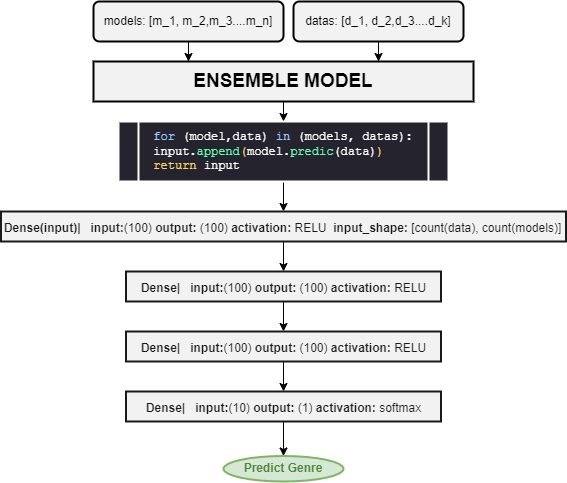
\includegraphics[width=8cm]{ensemble.png}
	\caption{Modelo del ensemble}
\end{figure}
\textbf{\large Resultados}\\
Dado que la base de datos utilizada contiene una cantidad relativamente peque\~na de datos al entrenar los modelos base con solo un 56\% de los datos se obtuvieron los resultados: 

\begin{itemize}
\item mfcc-cnn: 0.61 test accuracy
\item wavelets: 0.60 test accuracy 
\end{itemize}

Al entrenar el modelo final con el 20\% de los datos restantes se obtuvo un accuray de 0.65, lo cual si bien no es mejor resultado que los modelos entrenados individualmente con un conjunto de datos m\'as amplio, es un resultado que nos indica que en trabajos futuros con datasets m\'as abarcadoras, o con una dataset ampliada que tenga suficientes datos para preentrenar bien los modelos base, el ensemble mejora los resultados de los modelos previamente entrenados aprendiendo de las fortalezas de cada uno de estos.

	\section{Wavelets}

La clasificaci\'on de g\'eneros basada en la Transformada de Fourier, utilizando MFCC y espectrogramas, se ha explorado con \'exito en los \'ultimos a\~nos. Aunque la Transformada de Fourier tiene una alta resoluci\'on en el dominio de la frecuencia, tiene una resoluci\'on cero en el dominio del tiempo. Esto significa que puede decirnos exactamente qu\'e frecuencias est\'an presentes en una se\~nal, pero no en qu\'e lugar en el tiempo se han producido \cite{wavelet transform in machine learning}. Un mejor enfoque para analizar se\~nales con un espectro de frecuencias din\'amico es la Transformada Wavelet. Esta tiene una alta resoluci\'on tanto en el dominio de la frecuencia como en el del tiempo. Adem\'as, la Transformada Wavelet puede proporcionar una resoluci\'on de frecuencia variable, lo que significa que puede adaptarse a diferentes escalas de tiempo y frecuencia. Esto puede ser \'util en la clasificaci\'on de g\'eneros musicales, donde ciertos g\'eneros pueden tener patrones r\'itmicos m\'as r\'apidos o lentos que otros \cite{Musical Genre Classification Of Audio Signals}. Por \'ultimo, la Transformada Wavelet, ya que utiliza pocos datos para representar una se\~nal puede ser \'util en la clasificaci\'on de g\'eneros musicales; donde el procesamiento de grandes cantidades de datos suele ser costoso en t\'erminos de tiempo y recursos computacionales. 

	Proponemos dos m\'etodos de extracci\'on de caracter\'isticas usando varias formas de Transformadas Wavelet. 
    El primero es la Transformada Wavelet Discreta (DWT) \cite{wavelet transform in machine learning} y el segundo la Transformada Wavelet Compleja de Doble \'arbol (DT-CWT) \cite{DT-CWT}.
    
    La DWT es un caso especial de Transformada Wavelet que proporciona una representaci\'on compacta de la se\~nal en el tiempo y la frecuencia que se puede calcular de manera eficiente\cite{Musical Genre Classification Of Audio Signals}. La DT-CWT es una mejora relativamente reciente a DWT; ya que para se\~nales moduladas complejas como el audio, DWT encuentra algunas pocas deficiencias: oscilaciones, varianza de desplazamiento, aliasing y falta de direccionalidad\cite{Wavelet Transform for Music Genre Classification}. 
    
    El pipeline para ambos m\'etodos consiste en calcular las respectivas caracter\'isticas para cada canci\'on del dataset. Luego con la matriz obtenida se realiza un split de $80\%$ - $20\%$ y se entrena el modelo de machine learning elegido. Ajustando los hiperpar\'ametros utilizando Cross-Validation.

	\subsection{Tests}

  Fueron probados varios modelos de machine learning tradicionales como Logistic Regression, SVC, Linear SVC, Random Forest Classifier y Gradient Boosting Classifier. Como los dos \'ultimos se comportan mejor respecto al resto, con una precisi\'on superior en un 10\%, decidimos enfocarnos en esos modelos . 

Respecto a la Transformada Wavelet Discreta, Daubechies wavelet  emp\'iricamente muestra el mejor comportamiento en muchas aplicaciones\cite{Wavelet Transform for Music Genre Classification}. Experimentamos con distintos \'ordenes de Daubechies wavelet, y db12 mostr\'o el mejor comportamiento. Los mejores resultados para DWT fueron obtenidos con Random Forest; utilizando como par\'ametros: \emph{n\_estimators=100}, \emph{max\_depth=13}, \emph{bootstrap=False}. La precisi\'on con este modelo se ubicaba alrededor de $0.77$. \\

	\begin{figure}[h!] % Start the main figure environment
		\centering
		\begin{subfigure}{0.45\linewidth} % First subfloat environment
			\includegraphics[width=4cm]{images/CV_DWT_gb.png}
			\caption{DWT Gradient Boosting}
		\end{subfigure}
		\begin{subfigure}{0.45\linewidth} % Second subfloat environment
			\includegraphics[width=4cm]{images/CV_DWT_rf.png}
			\caption{DWT Random Forest}
		\end{subfigure}
		\caption{DWT Cross-Validation}
	\end{figure}

La Transformada Wavelet Compleja de Doble \'arbol, mostr\'o los mejores resultados con 17 niveles de descomposici\'on para extraer los coeficientes wavelet. Se comporta mejor que DWT, alcanzando m\'as de $0.8$ de precisi\'on con Random Forest Classifier.  

Adem\'as de las imagenes del Cross-Vlidation tambi\'en reportamos una matriz de confusi\'on para comprobar el comportamiento en cada g\'enero. Se observa que no se desempe\~na de la misma forma en todos los g\'eneros, ya que hay algunos (como el metal o el jazz) donde se observan muy buenos resultados. \\

	\begin{figure}[h!] % Start the main figure environment
		\centering
		\begin{subfigure}{0.45\linewidth} % First subfloat environment
			\includegraphics[width=4cm]{images/CV_DTCWT_gb.png}                   
			\caption{DTCWT Gradient Boosting}
		\end{subfigure}
		\begin{subfigure}{0.45\linewidth} % Second subfloat environment
			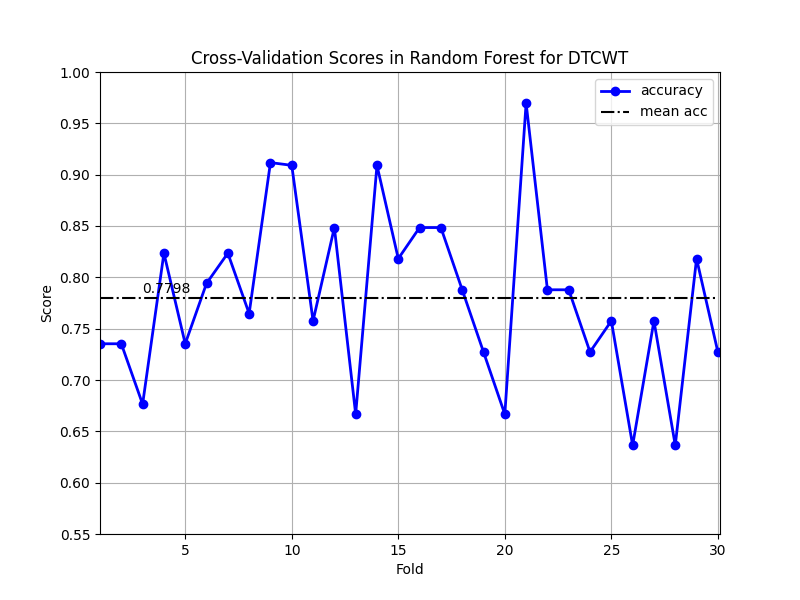
\includegraphics[width=4cm]{images/CV_DTCWT_rf.png}                  
			\caption{DTCWT Random Forest}
		\end{subfigure}
		\caption{DTCWT Cross-Validation}
	\end{figure}

\begin{figure}[h!] 
	\centering    
	\includegraphics[width=6cm]{images/conf_matrix_DTCWT.png}    
	\caption{DTCWT Random Forest Matriz de Confusi\'on}
\end{figure}

\section{Conv1D}
Implementamos un modelo de red neuronal convolucional unidimensional (CNN 1D) para clasificar g\'eneros de m\'usica. El modelo se basa en la arquitectura de ResNet, una popular red neuronal convolucional utilizada para tareas de clasificaci\'on. La elecci\'on de una red 1D permite al modelo procesar directamente se\~nales de audio, lo que lo hace especialmente \'util para esta tarea de clasificaci\'on de g\'eneros musicales.

\subsection{M\'etodo}
Lo interesante y diferente en este enfoque es que, en lugar de usar caracter\'isticas de audio pre-extra\'idas, el modelo aprende directamente de las formas de onda de audio. Esto puede resultar en un modelo m\'as flexible que puede aprender representaciones m\'as \'utiles para la tarea en cuesti\'on.

La idea principal del modelo es tomar una se\~nal de audio, pasarla a trav\'es de una serie de capas convolucionales para extraer caracter\'isticas \'utiles, y luego usar esas caracter\'isticas para clasificar la se\~nal en uno de los g\'eneros musicales.

El c\'odigo se divide en varias partes:
\begin{itemize}
\item Carga de archivos de audio: Se usa la biblioteca librosa para cargar los archivos de audio con una frecuencia de muestreo de 22050 Hz.
\item Preprocesamiento de los datos: Los g\'eneros se codifican en representaciones num\'ericas y los datos se dividen en conjuntos de entrenamiento, validaci\'on y prueba.
\item Construcci\'on del modelo: Se define un modelo de red neuronal convolucional 1D con varias capas, incluyendo capas convolucionales, una capa de agrupaci\'on (pooling), y una capa densa (fully connected).
\item Entrenamiento del modelo: El modelo se entrena en los datos de entrenamiento, utilizando una funci\'on de p\'erdida de entrop\'ia cruzada categ\'orica y el optimizador Adam.
\end{itemize}

\subsection{Comentarios}
Sin embargo, cabe mencionar que, aunque el modelo est\'a inspirado en la arquitectura ResNet, la implementaci\'on en el c\'odigo no incluye las conexiones de atajo (shortcut connections) que caracterizan a ResNet. Estas conexiones permiten que las se\~nales pasen directamente a trav\'es de la red, ayudando a combatir el problema del desvanecimiento del gradiente durante el entrenamiento de redes profundas. A pesar de la ausencia de estas conexiones, el modelo a\'un puede ser efectivo para la tarea de clasificaci\'on de g\'eneros de m\'usica. Los trabajos futuros podr\'ian considerar la implementaci\'on de las conexiones de atajo para recrear m\'as fielmente la arquitectura ResNet y potencialmente mejorar el rendimiento.

\subsection*{Integraci\'on en Google Colab}

El ensamblaje del modelo de entrenamiento que implementamos de Red Neuronal Convolucional 1D, o Conv1D, fue realizado en Google Colab. Este proceso fue necesario debido a la falta de recursos para el entrenamiento de la estructura de datos necesaria. Tambi\'en nos beneficiamos de la capacidad de Google Colab para manejar las multiplicaciones de inmensas matrices que se realizan durante los algoritmos de propagaci\'on hacia adelante y hacia atr\'as en el entrenamiento de la red.

El modelo es entregado en formato Jupyter Notebook (extensi\'on .ipynb), lo que facilita la claridad y separaci\'on en m\'odulos, as\'i como la ejecuci\'on de partes espec\'ificas del c\'odigo seg\'un sea necesario. Para una ejecuci\'on m\'as f\'acil del modelo, se recomienda ejecutar el notebook desde Google Colab. Esto agilizar\'a las descargas necesarias y evitar\'a la necesidad de instalar m\'odulos como 'tensorflow' y 'numpy', que ya est\'an incluidos en el entorno de ejecuci\'on de Python en Google Colab.

La ejecuci\'on y el entrenamiento del modelo se dividen en cuatro partes fundamentales:

\begin{enumerate}
\item Importaci\'on de la biblioteca 'os' de Python.
\item Sincronizaci\'on con Google Drive.
\item Descarga e importaci\'on del dataset GTZAN.
\item Entrenamiento del modelo.
\end{enumerate}

\subsection*{1. Importaci\'on de la biblioteca 'os' de Python}

La importaci\'on de la biblioteca 'os' de Python es necesaria para trabajar con el dataset de forma local despu\'es de la descarga.

\subsection*{2. Sincronizaci\'on con Google Drive}

La sincronizaci\'on con la cuenta de Google Drive nos permite trabajar con el dataset desde la nube, evitando la necesidad de descargarlo a nuestra PC. Una vez que se ejecuta el c\'odigo identificado en el notebook para este prop\'osito, nuestro almacenamiento en Google Drive ser\'a accesible.

\subsection*{3. Descarga e importaci\'on del dataset GTZAN}

El c\'odigo para descargar e importar el dataset GTZAN solo necesita ser ejecutado una vez. Despu\'es de descargar el dataset GTZAN, lo tendremos localmente para usarlo cuantas veces sea necesario.

La descarga se realiza desde Kaggle, una plataforma que proporciona una gran cantidad de datasets y ofrece una API que nos permite descargar casi todos ellos. Los pasos detallados para descargar el dataset GTZAN desde Kaggle se explican en el notebook.

\subsection*{4. Entrenamiento del modelo}

Inicialmente, concebimos el entrenamiento del modelo trabajando directamente con los audios. Sin embargo, al investigar la clasificaci\'on de g\'eneros musicales y trabajar con m\'usica en general, optamos por trabajar con histogramas de las canciones. Aunque dejamos ambos enfoques en el modelo, es importante solo ejecutar uno de los dos. Las instrucciones detalladas para el entrenamiento del modelo se encuentran en el notebook.

\section{Modelo VisionLang}

Hasta ahora hemos implementado algunas de las ideas m\'as exitosas para clasificar g\'eneros musicales que se pueden encontrar en el estado del arte. Pero resulta que ninguna de estas hace uso de la letra de la canci\'on, la cu\'al sabemos intuitivamente que puede aportar bastante informaci\'on sobre el g\'enero de la canci\'on. Por tanto, una idea implementada en este trabajo es hacer un modelo clasificador que conste de una red neuronal que combina an\'alisis de la letra, mediante un embedding que represente a la misma, y de la m\'usica con un encoder. La idea de este modelo es concatenar los vectores resultantes de estos procesamientos y clasificar en base a esta combinaci\'on de features. Al mismo lo llamamos como VisionLang.

\subsection{Feature: Letra de la canci\'on}

La segunda mitad de la informaci\'on de la que queremos que nuestro modelo aprenda es la letra de la canci\'on. Para ello lo primero que se hace es extraer la misma haciendo uso del conocido modelo de Whisper (ver \cite{whisper}). Luego necesitamos un embedding que represente al texto de la canci\'on que servir\'a de entrada al modelo. Para extraer el mismo hacemos uso de otro modelo de aprendizaje de m\'aquinas conocido como Bert (ver \cite{bert}). Este \'ultimo es un modelo basado en redes neuronales para el procesamiento de lenguaje natural, desarrollado por Google.

\subsection{Arquitectura del modelo}

Una vez obtenidos los dos embedding correspondientes a la letra de la canci\'on y la m\'usica (MFCC) ya tenemos la capa de entrada de nuestra red neuronal. La misma es la concatenaci\'on de los dos vectores obtenidos. Luego la red tiene  dos capas ocultas con funci\'on de activaci\'on RELU y cantidad de neuronas $128$ y $64$ respectivamente. Finalmente la capa de salida consiste de $10$ neuronas que representan a cada uno de los g\'eneros musicales que analizamos, y cuenta con softmax como funci\'on de activaci\'on. Siendo coherente con esto \'ultimo usamos como funci\'on de p\'erdida la Categorical Cross Entropy. Adem\'as, el modelo fue entrenado durante $500$ epochs.


\subsection{Resultados}

Como podemos ver en la siguiente gr\'afica el valor de accuracy de nuestro modelo para el training set es casi perfecto llegados al epoch n\'umero $300$. En el caso del conjunto de  datos de validaci\'on, que es el que nos da la efectividad de nuestro modelo, vemos que el accuracy crece r\'apidamente hasta llegar al valor $0.57$ alrededor del epoch $150$.

\begin{figure}[h!]
	\includegraphics[width=5cm]{vl_accuracy.png}
\end{figure}

Con m\'as capas y neuronas en nuestro modelo, este hac\'ia r\'apidamente overfitting, o sea en pocos epochs. Esto nos llev\'o a reducirlo a la arquitectura actual. Como podemos observar en la pr\'oxima gr\'afica la funci\'on de p\'erdida para los datos entrenantes decrece r\'apidamente acerc\'andose mucho a cero en el epoch $300$. En el caso de los datos de validaci\'on, vemos como a partir del epoch $100$ la red comienza a hacer overfitting, pero no es representativo. 

\begin{figure}[h!]
	\includegraphics[width=5cm]{vl_loss.png}
\end{figure}

%Presentamos aqu\'i adem\'as la matriz de confusi\'on.

\begin{figure}[h!]
	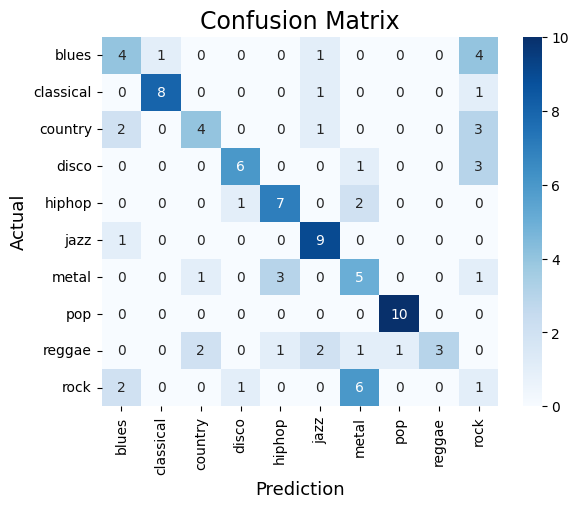
\includegraphics[width=5cm]{vl_confussion_matrix.png}
\end{figure}

Finalmente con un accuracy de $0.57$ y con valor para la funci\'on de p\'erdida de  $2.9323$ llegamos a la conclusi\'on de que este modelo no arroja resultados que mejoren los obtenidos en los modelos ya vistos antes.

	\section{Recomendaciones}
  
Un aspecto cr\'itico que afecta el rendimiento de los modelos de clasificaci\'on radica en la precisi\'on y consistencia de las anotaciones asignadas manualmente. Los esfuerzos futuros deber\'ian priorizar la recopilaci\'on de datos de mayor calidad a trav\'es de pautas m\'as estrictas, anotaciones de expertos o procedimientos de ratificaci\'on de colaboraci\'on colectiva.

Otro enfoque para impulsar el rendimiento de los modelos de clasificaci\'on de g\'enero es combinar m\'ultiples modelos a trav\'es de ensembles. Al integrar predicciones de distintos algoritmos y representaciones de caracter\'isticas, los ensembles aprovechan las fortalezas de los clasificadores individuales mientras mitigan sus debilidades.  

  Al seguir estas direcciones, los investigadores pueden ampliar nuestra comprensi\'on de la clasificaci\'on de g\'eneros musicales y sentar bases s\'olidas para soluciones de pr\'oxima generaci\'on en \'areas relacionadas, incluido el an\'alisis de audio, la recuperaci\'on de informaci\'on o las interfaces interactivas centradas en el ser humano.
  
	    
	\begin{thebibliography}{20}
		\bibitem{whisper} A. Radford, J. Wook Kim, T. Xu, G. Brockman, C. McLeavey y I. Sutskever: \emph{RobustSpeechRecognitionviaLarge-ScaleWeakSupervision}. Preprint on arXiv: 2212.04356, 2022. 	
		\bibitem{Conv1D} Safaa Allamy, Alessandro Lameiras Koerich: \emph{1D CNN Architectures for Music Genre Classification}. Preprint on arXiv.2105.07302, 2021. 
		\bibitem{bert} J. Devlin, M. Chang, K. Lee y K. Toutanova: \emph{BERT:Pre-trainingofDeepBidirectionalTransformersfor LanguageUnderstanding}. Preprint on arXiv: 1810.04805, 2018. 
		\bibitem{murphy} Kevin P. Murphy: \emph{Machine Learning: A Probabilistic Perspective}. MIT Press, 2012.
		\bibitem{Wavelet Transform for Music Genre Classification} Pranav Vijaya Kumar Rao, Vishwas Nagesh Moolimani: \emph{ECG Analysis based feature extraction using Wavelet Transform for Music Genre Classification}, 2020. 
		\bibitem{wavelet transform in machine learning} Ahmet Taspinar: \emph{A guide for using the wavelet transform in machine learning}, unpublished. [Online]. Available: http://ataspinar.com/2018/12/21/a-guide-for-using-the-wavelet-transform-in-machine-learning/
		\bibitem{DT-CWT} Selesnick, I.W. and Baraniuk, R.G. and Kingsbury, N.C., \emph{The dual-tree complex wavelet transform}, 2005, IEEE Signal Processing Magazine, pp. 123-151.
		\bibitem{Wavelets y sus Aplicaciones} Liliana R. Castro, Silvia M.  Castro: \emph{Wavelets y sus Aplicaciones}, ler. Congreso Argentino de Ciencias de la Computaci\'on, pp. 195-204.
		\bibitem{Musical Genre Classification Of Audio Signals} George Tzanetakis, Georg Essl, Perry Cook: \emph{Automatic Musical Genre Classification Of Audio Signals}
		\bibitem{Machine Learning and Deep Learning methods for music genre Classification} Rusian Gohkman: \emph{Machine Learning and Deep Learning methods for music genre Classification}
		\bibitem{michelucci2022introduction} Umberto Michelucci: \emph{An Introduction to Autoencoders}. Preprint on arXiv: 2201.03898, 2022.
		\bibitem{bank2021autoencoders} Dor Bank and Noam Koenigstein and Raja Giryes: \emph{Autoencoders}. Preprint on arXiv: 2003.05991, 2021.
    \end{thebibliography}
	
\end{document}
